\documentclass[a4paper, 12pt]{article}
\usepackage[T1]{fontenc}
\usepackage[scale=1,angle=0,opacity=1,color=black!60]{background}
\usepackage{tikzpagenodes}
\usepackage{lastpage}
\usepackage{lmodern}
\usepackage{float}
\usepackage{adjustbox}
\usepackage{amsmath}
\usepackage{nccmath}
\usepackage{url}
\usepackage{listings}
\usepackage{alltt}
\usepackage[section]{placeins}
\usepackage{tocloft}
\renewcommand{\cftsecleader}{\cftdotfill{\cftdotsep}}  % lineas punteadas en la tabla de contenidos
%\newcommand\mydotfill{\cftdotfill{\cftdotsep}}

\usepackage[textwidth=420pt,textheight=630pt]{geometry}
\setlength{\oddsidemargin}{15.5pt}
%\usepackage[none]{hyphenat} %no cortar palabras

\usepackage[spanish, activeacute]{babel} %Definir idioma español
\usepackage[utf8]{inputenc} %Codificacion utf-8
\backgroundsetup{contents={}} %Saca el 'draft'
\definecolor{mygray}{rgb}{0.95,0.95,0.95}

\usepackage{listings}
\lstset{
    basicstyle=\footnotesize,
    backgroundcolor=\color{mygray},
    breaklines=true,
    breakatwhitespace=true,
    postbreak=\mbox{\textcolor{red}{$\hookrightarrow$}\space},
    captionpos=b,
    keepspaces=true,
    numbers=left,
    numbersep=5pt,
    showspaces=false,
    showstringspaces=false,
    showtabs=false,
    tabsize=4,
    language=C,
    frame=none,
	title=\lstname,
}

\def\labelitemi{$\bullet$}

\begin{document}
	% TÍTULO, AUTORES Y FECHA
	\begin{titlepage}
		\vspace*{\fill}
		\begin{center}
			\Large 75.10 Técnicas de diseño \\
			\Huge Trabajo Práctico 1: Validador de ofertas \\
			\textbf{Fecha de Entrega:} 3/10/2018\\
			\bigskip
			\begin{center}
				\begin{tabular}{||c | c||}
					\hline
					Integrantes & Padrón \\ [0.5ex]
					\hline\hline
					Augusto Arturi & 97498 \\
					\hline
					Pablo Inoriza & 94986 \\
					\hline
					Manuel Luis Llauró & 95736 \\
					\hline
					Sebastián Ezequiel Blanco & 98539 \\
					\hline
				\end{tabular}
			\end{center}

		\end{center}
		\vspace*{\fill}
	\end{titlepage}
	\pagenumbering{arabic}
	\newpage

	% ÍNDICE
	\tableofcontents
	\newpage
	\pagenumbering{arabic}

	\section{Modelo del dominio}
		\begin{figure}[ht]
			\begin{adjustbox}{addcode={
				\begin{minipage}{\width}}{
					\caption{%
						Modelo del dominio
						}
				\end{minipage}},rotate=360,center}
				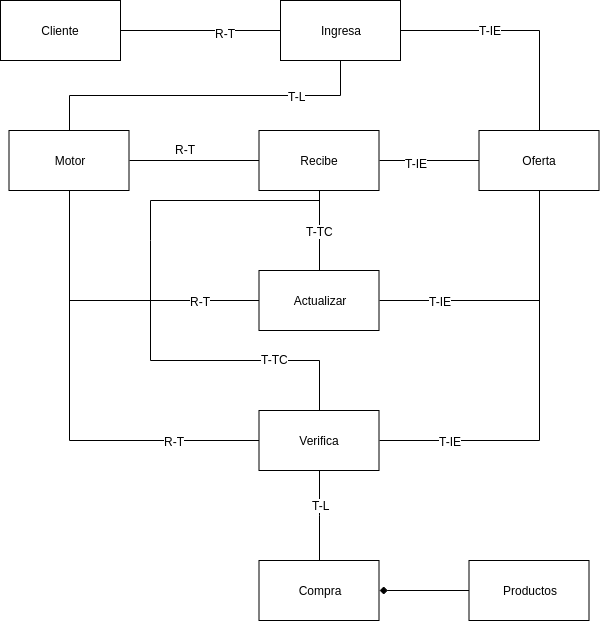
\includegraphics[scale=.6]{ModeloDominio.png}
			\end{adjustbox}
		\end{figure}
		\FloatBarrier
		\newpage

	\section{Explicacion de los modulos}
		% OFFER_PROCESSOR
		\subsection{offer\_processor}
			Este módulo es el principal del trabajo y contiene la interfaz pública que se provee al usuario, donde exiten dos 				funciones:\\
			\begin{lstlisting}[frame=tb, caption=firmas de la interfaz pública, label=zebra, tabsize=1]
				[state] initialize-offers [offers rules]
				[offers-applied] = process-sale [state, sale]
			\end{lstlisting}
			La primer función (initialize-offers) recibe una lista de ofertas y una lista de reglas y las almacena retornando un 				valor que representa una estado. \\
			La segunda función (process-sale) recibe el estado que se obtuvo de la función anterior y recibe una compra que 			contiene productos, un calendario y una forma de pago, retornando un vector donde cada elemento representa una oferta 				que aplico a la compra con el respectivo descuento.

		\newpage
		% OFFER_APPLIER
		\subsection{offer\_applier}
			Este módulo tiene una sola función que obra de interfaz pública y es la siguiente:
			\begin{lstlisting}[frame=tb, caption=firmas de la interfaz pública, label=zebra, tabsize=1]
				[offers-applied] = apply_offer [offer sale]
			\end{lstlisting}
			Esta función recibe una única oferta que se la aplica a la respectiva compra (sale) retornando un vector de mapas donde 				cada uno tiene el sigueinte formato:
			\begin{lstlisting}[frame=tb, caption=mapa resultado de ofertas aplicadas, label=zebra, tabsize=1]
				{
					"description" "una descripcion"
					"offer_code" "un codigo"
					"discount" "un valor"
				}
			\end{lstlisting}
			Cada oferta tiene un porcentaje de descuento y una compra tiene varios productos, por lo tanto en cada uno de estos 				mapas $"discount"$ es el valor que se descuenta por cada producto que cumple con la oferta.\\
			Luego tenemos funciones internas del módulo que resuelven otros problemas y las firmas son estas:
			\begin{lstlisting}[frame=tb, caption=firmas de las funciones privadas, label=zebra, tabsize=1]
				[products] get_products_that_met_the_rules [offer sale]
				[offers-applied] get_offer_result [offer products]
				[discount-value] apply_discount [offer price]
			\end{lstlisting}
			La primer función recibe una oferta y una compra y retorna una lista de productos los cuales cumplen con la oferta.
			Cada producto de este vector que retorna tiene un formato nuevo con un criterio propio. El formato de cada producto es 				cambiado dentro de esta función para facilitar el diseño del código y con un ejemplo mostramos como representamos un 				producto:
			\begin{lstlisting}[frame=tb, caption=formato de un producto, label=zebra, tabsize=1]
				{
					'products' {
						'name' 'Leche Descremada 1L, la Calmisima'
						'brand' {
							'code' 'Z001ABC'
							'name' 'La Calmisima'
						}
						'category' {
							'code' 'X033AXX'
							'name' 'Lacteo'
						}
						'price'  25.40
						'iva_porcentage' 10.5
						'code' 'X033XXX'
					}
					'payment' {
						'method' 'CASH'
						'bank' 'CAPRO'
					}
					'purchase_date' {
						'year' '2018'
						'month' 'SEPTEMBER'
						'day_number' 20
						'week_day' 'Thursday'
						'week_number' 4
					}
				}
			\end{lstlisting}
			La segunda función (get\_offer\_result) recibe una oferta y una lista de productos (con el formato ya explicado) que 				cumplen con dicha oferta y retorna un vector de oferta aplicadas cuyo formato de cada oferta aplicada se explicó 				anteriormente (ver Listing 3: mapa resultado de ofertas aplicadas).

		\newpage
		% RULE_APPLIER
		\subsection{rule\_applier}
			Este módulo tiene una sola función que obra de interfaz pública y es la siguiente:
			\begin{lstlisting}[frame=tb, caption=firmas de la interfaz pública, label=zebra, tabsize=1]
				[boolean-vector] = apply_rules [rules_codes prod]
			\end{lstlisting}
			Esta función recibe un vector de codigos de reglas y un producto con un formato explicado anteriormente
			(ver Listing 5: formato de un producto) y retorna un vector de boleano donde cada uno representa si el producto cumple 				o no con cada regla (true: cumple, false: no cumple).\\

			Luego tenemos funciones internas del módulo que resuelven otros problemas y las firmas son estas:
			\begin{lstlisting}[frame=tb, caption=firmas de las funciones privadas, label=zebra, tabsize=1]
				[rule] get_rule [rule_code]
				[boolean] atomic_rule [rule prod]
				[boolean] apply_atomic_rule [rule prod]
				[boolean-vector] multiple_rules [rules_codes prod]
				[boolean-vector] apply_multiple_rules [rules_codes prod]
			\end{lstlisting}
			La primer función (get\_rule) recibe el código de una regla y devuelve la regla.\\
			La segunda función (atomic\_rule) es un multimétodo el cual recibe una regla y un producto con un formato explicado 				anteriormente (ver Listing 5: formato de un producto) y devuelve un booleano que nos dice si el producto cumple o no 				con la regla. Esto es un multimétodo ya que no sabemos si la regla es atómica o es una regla con subreglas, por lo tanto
			si la regla es atómica ejecuta la función apply\_atomic\_rule, la cual recibe una regla atómica y un producto y retorna 			un boleano. Si la regla no es atómica llama a otro multimétodo que es multiple\_rules, que recibe una regla no atómica 				y el producto. Si la regla no atómica esta compuesta por una única subregla ejecuta apply\_atomic\_rule donde recibe la 				subregla y el producto. Si la regla no atómica esta compuesta por mas de una subregla ejecuta apply\_multiple\_rules 				donde recibe un vector de codigos de subreglas y el producto y retorna un vector de booleanos.

		\newpage
		% INSERTIONS
		\subsection{insertions}
			Este módulo tiene dos funciones que obran de interfaz pública y son las siguientes:
			\begin{lstlisting}[frame=tb, caption=firmas de la interfaz pública, label=zebra, tabsize=1]
				[nil] add_offer [o]
				[nil] add_rule [r]
			\end{lstlisting}
			La primer función recibe un vector de ofertas y lo almacena en una variable global llamada offers\_vector. Dentro de la 			función hace chequeos de datos y en caso de haber un dato inválido retorna excepción.\\
			La segunda función recibe un vector de reglas y lo almacena en una variable global llamada rules\_vector. Dentro de la 				función hace chequeos de datos y en caso de haber un dato inválido retorna excepción.\\
		\newpage
		% OPERATORS
		\subsection{operators}
			Este módulo tiene una función que obra de interfaz pública y es un multimétodo y es la siguiente:
			\begin{lstlisting}[frame=tb, caption=firmas de la interfaz pública, label=zebra, tabsize=1]
				[boolean] apply_op [op values field]
			\end{lstlisting}
			Esta función recibe un string (op) que representa la operación a realizar y dependiendo que tipo de operación values
			y/o field tomas distintos formatos. Si se quiere ejecutar las operaciones AND, OR, NOT , values sera un vector de 				boleanos al cual de le apicara dicha operación y field sera nil, ya que no se usara. Si se quiere ejecutar las 				operaciones LOWER, HIGHER, EQUALS values sera un valor singular y field tambien. Si se quiere ejecutar la operación IN, 			values sera un vector de valores y field sera un valor singular.

		\newpage
		% FIELDS
		\subsection{fields}
			Este módulo tiene una sola función que obra de interfaz pública y es la siguiente:
			\begin{lstlisting}[frame=tb, caption=firmas de la interfaz pública, label=zebra, tabsize=1]
				[field] get_field [product rule]
			\end{lstlisting}
			Esta función recibe un producto	con un formato explicado anteriormente (ver Listing 5: formato de un producto) y una 				regla y retorna el campo del producto el cual la regla especifica.\\

			Luego tenemos funciones internas del módulo que resuelven otros problemas y las firmas son estas:
			\begin{lstlisting}[frame=tb, caption=firmas de las funciones privadas, label=zebra, tabsize=1]
				[path] rule_field_path [rule]
				[key] translate [value])
			\end{lstlisting}
			La primer función recibe una regla y retorna un vector de claves de un mapa en el cual se encuetra el valor buscar en 				el producto.\\
			La segunda función es un multimétodo y recibe una clave que representa parte del camino (path) para encontrar el field 				y lo traduce a el nombre que el mapa usa, ya que por ejemplo las reglas usan la palabra CALENDAR para referirse al 				campo purchase\_date de un producto.

		\newpage
		% EXCEPTIONS
		\subsection{exceptions}
			Este módulo tiene cuatro funciones que obran de interfaz pública que son multimetodos y son las siguientes:
			\begin{lstlisting}[frame=tb, caption=firmas de la interfaz pública, label=zebra, tabsize=1]
				[field/Exception] check_field [field msg]
				[id/Exception] check_unknown_id [id]
				[rules/Exception] check_cycle_id [rules]
				[ids/Exception] check_duplicate_codes [ids code]
			\end{lstlisting}
			La primer función recibe un campo y un mensaje y si dicho campo es inválido, es decir tiene un valor que no esta 				permitido, retorna una excepción con el mensage. En caso contrario retorna el campo.\\
			La segunda función recibe un id que puede estar en formato json o no y si no contiene ningun dato o es un nill retorna 				excepción. En caso contrario retorna el id.\\
			La segunda función recibe un vector de reglas y si existen reglas no atomicas las cuales son ciclicas retorna una 				excepción. En caso contrario retorna las reglas.\\
			La segunda función recibe un vector ids que podrian ser tanto reglas como ofertas y si existen dos id con el campo code 			en el mismo valor retirna excepción. En caso contrario retorna las reglas.\\

		\newpage
		% CONVERTIONS
		\subsection{convertions}
			Este módulo tiene dos funciones que obran de interfaz pública y son las siguientes:
			\begin{lstlisting}[frame=tb, caption=firmas de la interfaz pública, label=zebra, tabsize=1]
				[structure] json_to_map [j]
				[json] map_to_json [j]
			\end{lstlisting}
			La primera función recibe un string (json) y lo retorna en la estructura de datos correspondiente de clojure.\\
			La segunda función recibe una estructura de datos clojure y la convierte en string (json).\\

		\newpage
		% TRANSLATIONS
		\subsection{translations}
			Este módulo tiene una sola función que obra de interfaz pública que es un multimétodo y es la siguiente:
			\begin{lstlisting}[frame=tb, caption=firmas de la interfaz pública, label=zebra, tabsize=1]
				[month] translate [month]
			\end{lstlisting}
			Esta función recibe un mes en español o ingles y lo retorna en español. Esto se debe a que la veces se termina 				comparando los mismos meses en distintos idiomas y la comparacion da falso, por lo tanto  no aseguramos de tener todo 				en un mismo idioma.

\end{document}
